\documentclass[./main.tex]{subfiles}
\graphicspath{{\subfix{images/}}}
\usepackage{multirow}
\begin{document}
	\section{Main chip}
	\subsection{IO addresses}
	\begin{center}
		\begin{tabular}{|c | c | c|}
			\hline
			Name & Mode & Address(hex) \\
			\hline
			Control register & w & f0 \\
			\hline
			Write data & w & f1 \\
			\hline
			Read data & r & f2 \\
			\hline
			Figure X coordinate & r/w & f3 \\
			\hline
			Figure Y coordinate & r/w & f4 \\
			\hline
			Score & r/w & f5 \\
			\hline
			Read keyboard & r & f6 \\
			\hline
			Read status & r & f7\\
			\hline
		\end{tabular}
	\end{center}
	Addresses 0xf0 to 0xf7 are reserved for I/O.  Addresses from 0xf8 to 0xff are reserved for the stack.
	\subsection{Control register}
	
	\subsection{Keyboard}
	\begin{figure}[h]
		\centering
		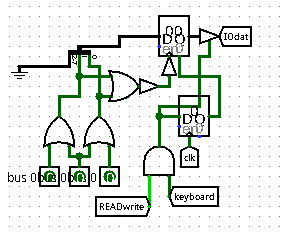
\includegraphics[width=8cm]{keyboard}
		\label{fig:img2}
		\caption{Keyboard}
	\end{figure}
	This part of the chip has 3 inputs, each of which is responsible for the movement of the figure: left, turn, right. When one of the inputs receives a logical unit, the value corresponding to the purpose of the input is written to the register in accordance with the table. The register value is cleared after the Cdm-8 reads its value.
	\begin{center}
		\begin{tabular}{|p{3cm}|p{3cm}|p{3cm}|}
			\hline
			\multicolumn{3}{|c|}{Bit mask} \\
			\hline
			left & rotate & right \\
			\hline
			0b00000010 & 0b00000011 & 0b00000001 \\
			\hline
		\end{tabular}
	\end{center}
\end{document}